\section{Informal development}
\label{sec:intuition}

We illustrate  all four new reasoning principles of \colosl by
sketching a proof of a simple, if slightly artificial,  example. 
We will look at less contrived examples in
\S\ref{sec:examples}. Consider the program $\mathbb{INC}$ defined
in Figure~\ref{.}, ignoring the assertions. It is written in pseudo-code, where variables $x$, $y$ and $z$ are allocated
on the heap and variable reading and mutation are understood as the
corresponding heap operations. After initialisation of the variables
to $0$, three threads are spawned to increment each variable in a
lock-step fashion: $\mathbb{P}_x$ is the first allowed to run its
increment operation; then $\mathbb{P}_y$;  and finally
$\mathbb{P}_z$. This process repeats until $x = y = z = 10$.
This example code is interesting because the threads are intrically
intertwinned. Why else interesting?.....The programmer knows......

\begin{figure*}
\centering
\begin{tabular}{@{}l@{\ }|@{\ }l@{\ }|@{\ }l@{\ }|@{\ }l@{}}
  {$\mathbb{P}_x$:}& 
  {$\mathbb{P}_y$:}& 
  {$\mathbb{P}_z$:}&
  $\mathbb{INC}$:\\[.5ex]
\begin{lstlisting}
//$\comment\{\shared{\cell{z}{0} * \cell{x}{0}}{I_x} * \token a_x\}$
while($x$ != 10)
//$\comment\left\{\shared{\begin{array}{@{}l<{\null}@{}l<{\null}@{}}\exsts{v}\cell{z}{v} * \cell{x}{v} \lor\\ \cell{z}{v} * \cell{x}{v+1}\end{array}}{I_x}\!\!\!\!\!\! * \token a_x\right\}$
{ $\langle$if ($x$ == $z$) $x$++;$\rangle$ }
//$\comment\left\{\shared{\begin{array}{@{}l<{\null}@{}l<{\null}@{}}\cell{z}{10} * \cell{x}{10} \lor\\ \cell{z}{9} * \cell{x}{10}\end{array}}{I_x}\!\!\!\!\!\! * \token a_x\right\}$
\end{lstlisting}
&
\begin{lstlisting}
//$\comment\left\{\shared{\begin{array}{@{}l<{\null}@{}l<{\null}@{}}\cell{x}{0} * \cell{y}{0} \lor\\ \cell{x}{1} * \cell{y}{0}\end{array}}{I_y}\!\!\!\!\!\! * \token a_y\right\}$
while($y$ != 10)
//$\comment\left\{\shared{\begin{array}{@{}l<{\null}@{}l<{\null}@{}}\exsts{v}\cell{x}{v} * \cell{y}{v} \lor\\ \cell{x}{v+1} * \cell{y}{v}\end{array}}{I_y}\!\!\!\!\!\! * \token a_y\right\}$
{ $\langle$if ($y$ < $x$) $y$++;$\rangle$ }
//$\comment\left\{\shared{\begin{array}{@{}l<{\null}@{}l<{\null}@{}}\cell{x}{10} * \cell{y}{10} \lor\\ \cell{x}{11} * \cell{y}{10}\end{array}}{I_y}\!\!\!\!\!\! * \token a_y\right\}$
\end{lstlisting}
&
\begin{lstlisting}
//$\comment\left\{\shared{\begin{array}{@{}l<{\null}@{}l<{\null}@{}}\cell{y}{0} * \cell{z}{0} \lor\\ \cell{y}{1} * \cell{z}{0}\end{array}}{I_z}\!\!\!\!\!\! * \token a_z\right\}$
while($y$ != 10)
//$\comment\left\{\shared{\begin{array}{@{}l<{\null}@{}l<{\null}@{}}\exsts{v}\cell{y}{v} * \cell{z}{v} \lor\\ \cell{y}{v+1} * \cell{z}{v}\end{array}}{I_z}\!\!\!\!\!\! * \token a_z\right\}$
{ $\langle$if ($z$ < $y$) $z$++;$\rangle$ }
//$\comment\left\{\shared{\begin{array}{@{}l<{\null}@{}l<{\null}@{}}\cell{y}{10} * \cell{z}{10} \lor\\ \cell{y}{11} * \cell{z}{10}\end{array}}{I_z}\!\!\!\!\!\! * \token a_z\right\}$
\end{lstlisting}
&
\begin{lstlisting}
//$\comment\{x|-> - * y|-> - * z|-> - \}$
$x$ = 0; $y$ = 0; $z$ = 0;
//$\comment\{x|-> 0 * y|-> 0 * z|-> 0 \}$
//$\comment\left\{\begin{array}{@{}l<{\null}@{}l<{\null}@{}}\shared{x|-> 0 * y|-> 0 * z|-> 0} I\\ \null*\token a_x * \token a_y * \token a_z\end{array}\right\}$
($\mathbb{P}_x$ || $\mathbb{P}_y$ || $\mathbb{P}_z$)
//$\comment\left\{\begin{array}{@{}l<{\null}@{}l<{\null}@{}}\shared{x|-> 10 * y|-> 10 * z|-> 10} I\\ \null*\token a_x * \token a_y * \token a_z\end{array}\right\}$
\end{lstlisting}
\end{tabular}

\begin{minipage}{.2\textwidth}
\begin{align*}
  I_x &\eqdef \left\{
  \begin{array}{@{}l@{}}
    \token a_x:\, \exsts{v} \cell{z}{v} * \cell{x}{v}  \swap  \cell{z}{v} * \cell{x}{v+1}\\
    \token a_z:\, \exsts{v} \cell{x}{v+1} * \cell{y}{v+1} * \cell{z}{v}\swap \cell{x}{v+1} * \cell{y}{v+1} * \cell{z}{v+1}
  \end{array}
  \right.\\
  I_y &\eqdef \left\{
  \begin{array}{@{}l@{}}
    \token a_x:\, \exsts{v} \cell{x}{v} * \cell{y}{v} * \cell{z}{v}  \swap  \cell{x}{v+1} * \cell{y}{v} * \cell{z}{v}\\
    \token a_y:\, \exsts{v} \cell{x}{v+1} *  \cell{y}{v}\swap \cell{x}{v+1} * \cell{y}{v+1}
  \end{array}
  \right.\\
  I_z &\eqdef \left\{
  \begin{array}{@{}l@{}}
    \token a_y:\, \exsts{v} \cell{x}{v+1} * \cell{y}{v} * \cell{z}{v}  \swap \cell{x}{v+1} * \cell{y}{v+1} * \cell{z}{v}\\
    \token a_z:\, \exsts{v} \cell{y}{v+1} *  \cell{z}{v}\swap \cell{y}{v+1} * \cell{z}{v+1}
  \end{array}
  \right.
\end{align*}
\end{minipage}\quad\ 
\begin{minipage}{.2\textwidth}
\begin{align*}
  I &\eqdef \left\{
  \begin{array}{@{}l@{\,}l@{}l@{}}
    \token a_x: & \exsts{v} & \cell{z}{v} * \cell{x}{v} \swap\\
    &&\quad \cell{z}{v} * \cell{x}{v+1}\\
    \token a_y: & \exsts{v} & \cell{x}{v+1} * \cell{y}{v} \swap \\
    &&\quad \cell{x}{v+1} * \cell{y}{v+1}\\
    \token a_z: & \exsts{v} & \cell{y}{v+1} * \cell{z}{v} \swap \\
    &&\quad \cell{y}{v+1} * \cell{z}{v+1}
  \end{array}\right.
\end{align*}
\end{minipage}

\vspace{5pt}\hrule\vspace{5pt}
\caption{The concurrent increment program together with a \colosl proof
  sketch. Lines starting with \lstinline{//} contain formulas that describe
  the local state and the subjective shared state at the relevant program point.}
\label{fig:concurrentInc}
\end{figure*}

\pgcomment{I need line numbers on INC and Py to describe
  properly. need [x] all over the place.} 



Now, consider the \colosl assertions associated with $\mathbb{INC}$.
\colosl assertions comprise of fairly standard assertions from the
separation-logic literature~\cite{rey02,sepish,variablesasresource},
plus {\em subjective views} and {\em capability} assertions. \colosl
assertions are interpreted over a particular domain which includes:
{\em thread-local} state exclusively visible to the thread; {\em one}
global shared state accessible by all threads; and {\em  interference
actions}  describing how the global state can be updated. The
subjective views describe {\em partial} information about the global
shared state. The capability assertions give a thread the capability
to change that partial shared state.




After
initialisation, line~?? of $\mathbb{INC}$  provides a standard assertion stating that 
the thread-local state consists of three  heap cells,  which are referred to by  $x$,
$y$ and $z$ and contain the value  $0$. This resource in the thread-local state is
fully owned by  the thread. Using the extension axiom, the thread is able to give up  this local
resource and transfer it  to the global shared state. For example, line~?? demonstates the
creation of a subjective view $\shared{x|-> 0 * y|-> 0 * z|->
  0}I$. This assertion states that {\em part} of the underlying
global shared state now contains the three heap cells, with 
interference relation $I$ declaring  how  this shared state  is able 
change. For example,  the action 
\[
\token a_x:  \exsts{v}  \cell{z}{v} * \cell{x}{v} \swap
    \cell{z}{v} * \cell{x}{v+1}
\]
describes how, when the value of the heap cells given  by   $x$
and $z$ have the same value $v$, then the value for $x$ can be updated
to $v+1$. This is only possible when the
local state of a thread has the {\em capability} $\token a_x$. For  this
particular 
example, the assertion in line~?? simply has all the capabilities $\token
a_x * \token a_y * \token a_z$   in the local state; in general,
capablities can be buried inside boxes, only to emerge as a
consequence of an action
(see  ...). 

\begin{figure}
\centering
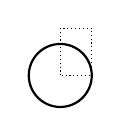
\begin{tikzpicture}
\draw[thick] (0,0) circle (.4cm);
\draw[densely dotted] (0,0) rectangle (.4cm,.6cm);
\end{tikzpicture}
\quad$\swap$\quad

\begin{tikzpicture}
\draw[thick] (0,0) circle (.4cm);
\draw[thick,fill=white] (0,0) rectangle (.6cm,.4cm);
\end{tikzpicture}\\


\null\hfill

\begin{tikzpicture}[baseline,yshift=.1cm]
\draw[thick] (0,0) circle (.4cm);
\end{tikzpicture}\quad subjective state
\hfill
$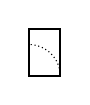
\begin{tikzpicture}[baseline,yshift=-.25cm]
\draw[thick] (0,0) rectangle (.4cm,.6cm);
\draw[densely dotted] (.4cm,0) arc (0:90:.4cm);
\end{tikzpicture}|= P$
\hfill
$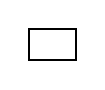
\begin{tikzpicture}[baseline]
\draw[thick,yshift=-.1cm] (0,0) rectangle (.6cm,.4cm);
\end{tikzpicture}|= Q$
\hfill\null

\vspace{5pt}\hrule\vspace{5pt}
\caption{Effect of an action $P\swap Q$.}
\label{fig:action}
\end{figure}



\pgcomment{next bit somewhere else}





A particularity of \colosl is that actions can be performed by the
environment any time their precondition is \emph{compatible} with the
current subjective state, and not only when the precondition is
satisfied by a \emph{substate} of the subjective state (as is required
for the program to perform the action). When that is the case, the
piece of state corresponding to the overlap between the state and the
precondition of the action is removed, and the entire postcondition of
the action is added in its place, as represented schematically in
\fig\ref{fig:action}.  In particular, an action whose precondition is
satisfiable is \emph{always} enabled from the empty subjective view
(which by definition is compatible with all other states).

Assertions appearing in pre and postconditions of triples must be
\emph{stable}. That is, for any action permitted by $I$, where $I$ is
the interference relation of a subjective view appearing in the
assertion, if the current thread does not exclusively hold the
associated capability (and thus the action may be performed by the
environment at any time), the assertion must remain true after the
action has taken place (see \fig\ref{fig:action}). For instance, the
assertion
\[
\token a_x * \token a_y * \shared{x|->0 * y|->0}{I_y}
\]
is stable since it owns the capabilities associated with both actions
of $I_y$ ($\token a_x$ and $\token a_y$), hence no other thread can
perform an action that would invalidate $x|->0 * y|->0$. On the other
hand, the assertion
\[
\token a_y * \shared{x|->0 * y|->0}{I_y}
\]
is not stable since a thread in possession of $\token a_x$ can
potentially increment the value of $x$ and thus invalidate $x|->0 *
y|->0$. A weaker, stable version of this assertion is the precondition
of $\mathbb P_y$.


%%%%%%%%%%%%%%%%%%%%%%%%%%%%%%%%%%
\subsection{Thread-local proofs}
\label{subsec:threads}

The proofs that $\mathbb P_x$, $\mathbb P_y$, and $\mathbb P_z$
satisfy the assertions at each program point as shown in
\fig\ref{fig:concurrentInc} are straightforward using standard
techniques from concurrency reasoning. In particular, commands in
angle brackets represent \emph{atomic sections}. Since all such
sections are operationally mutually exclusive, the program may safely
manipulate contents of the subjective region when executing an atomic
command. Logically, this translates into the following proof rule,
borrowed from concurrent abstract predicates~\cite{cap-ecoop10} (CAP):
\[
\infrule{Atomic}
        {\hoare p {\mathbb P} q\\
          \repartitions{P}{Q}{p}{q}}
        {\hoare P {<<\mathbb P>>} Q}
        {}
\]
\julescomment{TODO: explain rule}

Pleasingly, the thread-local proofs are only concerned with very
minimal subjective views of the state: the specification of each
thread only talks about the variables relevant to that thread, and
need only consider interferences that affect those variables, even
though the program as a whole operates on all three variables in a
fundamentally interdependent fashion. What may seem of little
consequence for this simple program (reasoning about the whole global
state would produce comparably short proofs in this example) is of
crucial importance when analysing larger systems, where the burden of
carrying the whole shared state around to analyse all threads, even
those that use only a small fraction of it, can lead to intractable
proofs. Subjectivity also enables the analysis of portions of code
without access to the whole program, and allows one to reuse the
established specifications in any environment that doesn't violate
their subjective views.

The three thread-local proofs are tied together in the main program
$\mathbb{INC}$ using two applications of the following concurrency
rule, as is standard in the concurrent separation logic family:
\[
\infrule{Parallel}
        {\hoare{P_1}{\mathbb{P}_1}{Q_1}\\
          \hoare{P_2}{\mathbb{P}_2}{Q_2}}
        {\hoare{P_1 * P_2}{\mathbb{P}_1 || \mathbb{P}_2}{Q_1 * Q_2}}
        {}
\]
More precisely, we will use the derivation below, starting from the
program state before the parallel composition and ending in the
$*$-conjunction of the preconditions of the thread threads, as
mandated by the \infrulestyle{Parallel} rule. The next sections are
devoted to justifying informally the various reasoning steps
involved. We let
\[
P_0 == x|-> 0 * y|->0 * z|-> 0
\]
and delay the definitions of $I_x'$, $I_y'$ and $I_z'$ until
\S\ref{subsec:shift}. Below, the unlabelled step is a simple logical
weakening of the boxed assertions, necessary to obtain stable
assertions as the preconditions of all threads.
\allowdisplaybreaks
\begin{align*}
  &\shared{P_0}{I} *\token a_x * \token a_y * \token a_z\\
  =>\null&
    (\shared{P_0}{I} *\token a_x)*
    (\shared{P_0}{I} *\token a_y)*
    (\shared{P_0}{I} *\token a_z)
  &\qquad\eqref{eq:split}\\
  =>\null&
  (\shared{P_0}{I_x'} *\token a_x)*
  (\shared{P_0}{I_y'} *\token a_y) *
  (\shared{P_0}{I_z'} *\token a_z)
  &\eqref{eq:shift} \\
  =>\null&
  \begin{array}[t]{L}
    (\shared{z|-> 0 * x|-> 0}{I_x'} *\token a_x)*\\
    (\shared{x|-> 0 * y|-> 0}{I_y'} *\token a_y)*
    \mathrlap{(\shared{y|-> 0 * z|-> 0}{I_z'} *\token a_z)}
  \end{array}
  &\eqref{eq:forget} \\
  =>\null&
  \begin{array}[t]{L}
    (\shared{z|-> 0 * x|-> 0}{I_x} *\token a_x)*\\
    (\shared{x|-> 0 * y|-> 0}{I_y} *\token a_y)*
    \mathrlap{(\shared{y|-> 0 * z|-> 0}{I_z} *\token a_z)}
  \end{array}
  &\eqref{eq:shift} \\
  =>\null&
  \begin{array}[t]{L}
    (\shared{\cell{z}{0} * \cell{x}{0}}{I_x} * \token a_x) *\\
    \left(\shared{\begin{array}{@{}l<{\null}@{}l<{\null}@{}}\cell{x}{0} *
        \cell{y}{0} \lor\\ \cell{x}{1} *
        \cell{y}{0}\end{array}}{I_y}\!\!\!\!\!\! * \token a_y\right) *
    \mathrlap{\left(\shared{\begin{array}{@{}l<{\null}@{}l<{\null}@{}}\cell{y}{0} *
        \cell{z}{0} \lor\\ \cell{y}{1} *
        \cell{z}{0}\end{array}}{I_z}\!\!\!\!\!\! * \token a_z\right)}
  \end{array}
\end{align*}

Conversely, going from the postconditions of the three threads to the
final state of $\mathbb{INC}$ is justified by the following reasoning
steps. We write $\shared{Q_x}{I_x} * \token a_x$ for the postcondition
of $\mathbb P_x$ as shown in \fig\ref{fig:concurrentInc}, and
similarly for $\mathbb P_y$ and $\mathbb P_z$.
\begin{align*}
  &(\shared{Q_x}{I_x} * \token a_x)
  * (\shared{Q_y}{I_y} * \token a_y)
  * (\shared{Q_z}{I_z} * \token a_z)\\
  =>\null&
  \shared{Q_x ** Q_y ** Q_z}{I_x\cup I_y\cup I_z} *
  \token a_x * \token a_y * \token a_z
  &\quad\eqref{eq:merge}\\
  =>\null&
  \shared{x|->10 * y|->10 * z|->10}{I_x\cup I_y\cup I_z} *
  \mathrlap{\token a_x * \token a_y * \token a_z}\\
  =>\null&
  \shared{x|->10 * y|->10 * z|->10}{I} *
  \token a_x * \token a_y * \token a_z
  &\eqref{eq:shift}
\end{align*}
Above, the unlabelled step is mere logical consequence, using the fact
that $|/$ distributes over $**$ and combining the knowledge of all
threads to get rid of spurious disjuncts (such as $x|-> 11 * y|->10$
in $Q_y$, when in fact we know from $Q_x$ that $x|->10$). Note
moreover that, \textit{e.g.},
\[
\begin{array}{RL}
&(\cell{z}{10} * \cell{x}{10}) ** (\cell{x}{10} * \cell{y}{10})\\
<=>&
\cell{x}{10} * \cell{y}{10} * \cell{z}{10}
\end{array}
\]



%%%%%%%%%%%%%%%%%%%%%%%%%%%%%%%%%%%%%%%%%
\subsection{Combining subjective views}
\label{subsec:merge}

As we have seen, a shared state assertion $\shared{P}{I}$ defines
contents of parts of the shared state only. A central property of
\colosl proofs is that multiple threads can view different,
potentially overlapping parts of the shared state. As such, the
separating conjunction $*$ behaves as \emph{overlapping conjunction}
$\sepish$~\cite{rey-slnotes,ramification} (sometimes called
\emph{sepish}~\cite{gareth-js12}) over subjective states (in contrast
with most existing formalisms, which would use \emph{classical
  conjunction} instead).
\begin{align*}
  \shared{P}{I} &=> \shared{P}{I} * \shared{P}{I}
  \tag{\textsc{Split}}\label{eq:split}\\
  \shared{P}{I_1} * \shared{Q}{I_2} &=> \shared{P \sepish Q}{I_1\cup I_2} \tag{\textsc{Merge}}\label{eq:merge}
\end{align*}
On local states, $*$ behaves as \emph{disjoint union}, as is standard.

\julescomment{This is actually two rules! Fix the words.}

This directly justifies the \eqref{eq:split} and \eqref{eq:merge}
steps of the two derivations above.


%%%%%%%%%%%%%%%%%%%%%%%%%%%%%%%%%%%%%%
\subsection{Forgetting shared state}
\label{subsec:forget}

In \colosl\ it is always possible to forget parts of the shared state
and arrive at a more subjective, and thus weaker, view of the shared
state. That is,
\begin{align}
  \label{eq:forget}
  \shared{P * Q}{I} &=> \shared{P}{I}  \tag{\textsc{Forget}}
\end{align}
It is straightforward to justify the \eqref{eq:forget}-labelled steps
of the derivations of \S\ref{subsec:threads} using this principle.

Note that, in the implication above, the right-hand-side is not
necessarily stable with respect to $I$. This is why we first make $I$
more explicit using~\eqref{eq:shift} in the derivation of
\S\ref{subsec:merge} (see below). Had we used~\eqref{eq:forget} at the
second step instead, we would have gotten
\[
\begin{array}[t]{L}
  (\shared{z|-> 0 * x|-> 0}{I} *\token a_x)*\\
  (\shared{x|-> 0 * y|-> 0}{I} *\token a_y)*
  (\shared{z|-> 0 * x|-> 0}{I} *\token a_z)
\end{array}
\]
where we no longer know the value of $y$ in relation to $x$ and $z$ in
the first conjunct $\shared{z|-> 0 * x|-> 0}{I} *\token a_x$, for
instance. Hence the action associated with capability $\token a_z$ can
now be carried out by the environment and change the value of $z$ at
any point in time according to $I$, and a stable assertion
corresponding to the first conjunct would have to be at least as weak
as
\[
\shared{\exsts{v, v'}  \cell{z}{v'} * \cell{x}{v}}{I}
\]
This is too weak to prove the spec of our program, since the
relationship between the values of $x$ and $z$ has been lost.



%%%%%%%%%%%%%%%%%%%%%%%%%%%%%%
\subsection{Action shifting}
\label{subsec:shift}

We now show how to use \colosl to change $I$ into $I_x$, $I_y$, and
$I_z$ before the parallel composition and $I_x\cup I_y\cup I_z$ into
$I$ afterwards, as in the two derivations of
\S\ref{subsec:threads}. This is all accomplished by the
\emph{interference shifting} mechanism of \colosl, which allows one to
rewrite the current inteference relation according to syntactic and
semantic deductions.  As mentioned in the introduction, the
corresponding logical principle takes the form
\begin{align}
  \label{eq:shift}
  I \weakenIb{P} I'
  &\text{ implies }
  \shared{P}{I} ===> \shared{P}{I'}
  \tag{\textsc{Shift}}
\end{align}
We will formalise the relation $\weakenIb{}$ in
\S\ref{sec:weakenI}. Let us illustrate it on our example.

Let us consider the action $\token a_z: \exsts{v} \cell{y}{v+1} *
\cell{z}{v} \swap \cell{y}{v+1} * \cell{z}{v+1}$ of $I$ and the state
$
\shared{P_0}{I}
$.
We notice that, anytime the precondition of $\token a_z$ is satisfied
in the shared state, then the larger formula $\exsts{v} \cell{x}{v+1}
* \cell{y}{v+1} * \cell{z}{v}$ is also satisfied, even after the
shared state has evolved from $x|-> 0 * y|-> 0 * z|-> 0$ using any
action in $I$. Thus, semantically, this action can be replaced with
the more precise
\[
\exsts{v}
\cell{x}{v+1} * \cell{y}{v+1} * \cell{z}{v}
\swap
\cell{x}{v+1} * \cell{y}{v+1} * \cell{z}{v+1}
\]
As we will see in \S\ref{sec:weakenI}, we can use this intuition and
similar reasoning for $I_y$ and $I_z$ to establish
\[
I\weakenIb{P_0} I_x'
\qquad
I\weakenIb{P_0} I_y'
\qquad
I\weakenIb{P_0} I_z'
\]
where
\begin{align*}
 I_x' &==
 \left[
   \token a_y <-
   \begin{array}{RL}
     \exsts{v}&\cell{x}{v+1} * \cell{y}{v} * \cell{z}{v} \swap\\
     &\cell{x}{v+1} * \cell{y}{v+1} * \cell{z}{v}
 \end{array}\right]I\\
 I_y' &==
 \left[
   \token a_z <-
   \begin{array}{RL}
     \exsts{v}&\cell{x}{v+1} * \cell{y}{v+1} * \cell{z}{v} \swap\\
     &\cell{x}{v+1} * \cell{y}{v+1} * \cell{z}{v+1}
   \end{array}\right]I\\
 I_z' &==
 \left[
   \token a_x <-
   \begin{array}{RL}
     \exsts{v}&\cell{x}{v} *\cell y v * \cell{z}{v}\swap\\
     &\cell{x}{v+1} * \cell{y}{v} * \cell z v
   \end{array}\right]I
\end{align*}

Now, consider for instance $\shared{x|->0 * y|->0}{I_y'}$.  The action
$\token a_z: \exsts{v} \cell{y}{v+1} * \cell{z}{v} \swap \cell{y}{v+1}
* \cell{z}{v+1}$ of $I_y'$ does not actually affect $x|->0 * y|->0$,
and never will in the lifetime of this subjective view (\textit{i.e.},
after any performing any number of actions from $I_y'$). Thus, it does
not matter semantically if this action this action is dropped from
$I_x'$, and similarly for $I_x'$ and $I_y'$:
\[
I_x'\weakenIb{P_0} I_x
\qquad
I_y'\weakenIb{P_0} I_y
\qquad
I_z'\weakenIb{P_0} I_z
\]

Using similar observations, we are able to make the deduction that
\[
I_x\cup I_y\cup I_z\weakenIb{x|->10 * y|->10 * z|->10} I
\]

This finishes the justification of all uses of \eqref{eq:shift} in the
derivations of \S\ref{subsec:threads}, and thus the derivations
themselves.  In this section, we have informally justified
manipulations of the interference relation by semantic
arguments. However, \S\ref{sec:shiftax} will show how the reasoning
involved can be reduced to simple logical implications between
separation logic formulas that do not mention the shared state.

%% In the case of the less local predicate $G$, whenever the
%% pre-condition of the action associated with $\token a_z$ is satisfied
%% (third disjunct), it is also the case that $\cell{x}{v+1}$. In other
%% words, in all the cases where the shared state satisfies
%% $\cell{y}{v+1} * \cell{z}{v}$, it also satisfies $\cell{x}{v+1} *
%% \cell{y}{v+1} * \cell{z}{v}$. However, this information is not
%% reflected in $I$ and as a result when weakening $G$, we need to
%% stabilise the resultant assertion which proves to be very weak. To
%% remedy this, in \colosl we introduce the notion of action
%% \emph{shifting} (rewriting) with respect to the \emph{invariant} of
%% the shared state. Given $\shared{P}{I'}$, we write $\fence{} \fences
%% (P, I')$ - read ``$\fence{}$ fences $P$ with respect to $I'$'' - to
%% indicate that i) $\fence{}$ contains all states associated with $P$
%% and ii) it is closed under $I'$; that is, given any action in $I'$
%% whose pre-condition is satisfied by a state in $\fence{}$, the state
%% resulting from the action is also in $\fence{}$. For instance, given
%% the $G$ predicate of \fig\ref{fig:concurrentIncCoLoSLSpec}, we have
%% $\fence{G} \fences (P_G, I)$ where $P_G$ denotes the assertion inside
%% the box and $\fence{G}$ is as specified below.
%% \[
%% 	\begin{array}{l l}
%% 		\fence{G} = \hspace*{-5pt}& \left\{\cell{x}{v} * \cell{y}{v} * \cell{z}{v} ||| v \in \{0, \cdots 10\} \right\} \\
%% 		& \cup \left\{\cell{x}{v+1} * \cell{y}{v} * \cell{z}{v} ||| v \in \{0, \cdots 9 \} \right\} \\
%% 		& \cup \left\{\cell{x}{v+1} * \cell{y}{v+1} * \cell{z}{v} ||| v \in \{0, \cdots 9\} \right\}\\
%% 	\end{array}
%% \]
%% %as well as the action associated with its update
%% Given the above invariant, we can now \emph{shift} the action associated with $\token a_z$ in $I$ and arrive at $I'$ where
%% \[
%% 	I' \eqdef \left\{
%% 		\begin{array}{@{}l@{}}
%% 			\token a_x:\, \exsts{v} \cell{x}{v} * \cell{z}{v}  \swap  \cell{x}{v+1} * \cell{z}{v}\\
%% 			\token a_y:\, \exsts{v} \cell{x}{v+1} * \cell{y}{v}  \swap  \cell{x}{v+1} * \cell{y}{v+1}\\
%% 			\token a_z:\, \exsts{v} \cell{x}{v+1} *
%%                         \cell{y}{v+1} * \cell{z}{v} \swap\null\\
%% 			\hspace*{2cm} \cell{x}{v+1} * \cell{y}{v+1} * \cell{z}{v+1}\\
%% 		\end{array}			
%% 	\right.
%% \]
%% Note that in doing so we have neither restricted nor relaxed the action of $\token a_z$ in that it can be carried out in exactly the same states given the invariant $\fence{G}$. This is formalised by the \textsc{(Shift)} rule where $I \weakenI{\fence{}} I'$ denotes the shifting of $I$ with respect to $\fence{}$ and we defer its formalisation to \S\ref{sec:logic}.
%% \[
%% 	\text{if}\hspace*{0.25cm} \fence{} \fences (P, I) 
%% 	\hspace*{0.25cm}\text{and}\hspace*{0.25cm} I \weakenI{\fence{}} I'
%% 	\hspace*{0.25cm}\text{then}\hspace*{0.25cm}
%% 	\shared{P}{I} ===> \shared{P}{I'} \hspace*{0.5cm} \textsc{(Shift)}
%% \]
%% Given predicate $G$ of \fig\ref{fig:concurrentIncCoLoSLSpec}, we can first shift $I$ into $I'$ (specified above) using the \textsc{Shift} rule and then apply the \textsc{Forget} rule to forget variable $y$ and obtain $\shared{a_x}{I'}$.
%% %%
%% %\[
%% %	X' \eqdef \shared{\exsts{v} \cell{x}{v} * \cell{z}{v} \lor \cell{x}{v+1} * \cell{z}{v}}{I'} 
%% %\]
%% %%
%% We have almost arrived at a local specification for $\mathbb{P}_x$. However, the action of $\token a_y$ is still visible in $I'$ even though it does not affect the values of $x$ or $z$. Through interference shifting, we can not only rewrite actions with respect to the invariant, we can also \emph{forget} actions that affect \emph{none} of the states contained in the invariant. For instance, let $\fence{x} = \left\{\cell{x}{v} * \cell{z}{v} ||| v \in \{0, \cdots 10\} \right\} \cup \left\{\cell{x}{v+1} * \cell{z}{v} ||| v \in \{0, \cdots 9 \} \right\}$, then we have $\fence{X} \fences (X, I')$. In the case of the action of $\token a_y$, given any state $p$ in the action pre-condition (e.g. $p = \cell{x}{1} * \cell{y}{0}$), for an arbitrary state $s \in \fence{X}$ (e.g. $s = \cell{x}{1} * \cell{z}{0}$), \emph{all overlaps} of $p$ and $s$ ($p \meetL s = \{\cell{x}{1}\}$) are preserved by the action. We give the formal definition of overlap operator $\meetL$ in \S\ref{sec:logic}. 

%% Given $I'$ and $\fence{X}$ we can again apply the \textsc{Shift} rule in order to forget about the action of $\token a_y$ and obtain $I_x$ as specified in \fig\ref{fig:concurrentIncSubjectiveSpec}. We can take analogous steps in order to obtain subjective views $S_y$ and $S_z$ for threads $\tau_y$ and $\tau_z$. We then pass the $\token a_x$, $\token a_y$ and $\token a_z$ capabilities to $\tau_x$, $\tau_y$ and $\tau_z$ and verify $\mathbb{INC}$ as follows:
%% \[
%% \hspace*{-0.2cm}
%% \begin{array}{c}
%% 	\color{blue}{\left\{\token a_x * \token a_y *  \token a_z *  S_x * S_y * S_z \right\}}\vspace*{2pt}\\
	
%% 	\begin{array}{c || c || c}
%% 		\color{blue}{\left\{\token a_x * S_x \right\}} & \color{blue}{\left\{\token a_y * S_y \right\}} & \color{blue}{\left\{\token a_z * S_z \right\}}\\
%% 		&&\vspace*{-7pt}\\
%% 		\mathbb{P}_x & \mathbb{P}_y & \mathbb{P}_z\\
%% 		&&\vspace*{-5pt}\\

%% 		\color{blue}{
%% 			\left\{
%% 					\token a_x * S'_x
%% 			\right\}
%% 		} 
%% 		& 
%% 		\color{blue}{
%% 			\left\{
%% 				\token a_y * S'_y
%% 			\right\}
%% 		} 

%% 		&
		
%% 		\color{blue}{
%% 			\left\{
%% 				\token a_z * S'_z
%% 			\right\}
%% 		} 		
%% 		\vspace*{3pt}
%% 	\end{array}\\
%% 	\color{blue}{\left\{\token a_x * \token a_y *  \token a_z *  S'_x * S'_y * S'_z \right\}}\\
%% \end{array}
%% \]
%% with
%% \[
%% \begin{array}{l l}
%% 	S'_x \eqdef & \shared{\cell{x}{10} * \cell{z}{10} \lor \cell{x}{10} * \cell{z}{9} }{I_x}\\
%% 	S'_y \eqdef & \shared{\cell{x}{11} * \cell{y}{10} \lor \cell{x}{10} * \cell{y}{10} }{I_y}\\
%% 	S'_z \eqdef & \shared{\cell{y}{11} * \cell{z}{10} \lor \cell{y}{10} * \cell{z}{10} }{I_z}
%% \end{array}
%% \]



%%%%%%%%%%%%%%%%%%%%%%%%%%%%%%%%%%%%%%%%%%
\subsection{Extending the shared region}
\label{subsec:extend}

All that remains to show is how the shared region is initially created
in $\mathbb{INC}$.  At the very beginning of the execution of
$\mathbb{INC}$, the state is purely local and contains the three
variables $x$, $y$, and $z$, which allows $\mathbb P$ to initialise
them to 0 without synchronisation. Since the purpose of the rest of
the program is to share these variables between $\mathbb P_x$,
$\mathbb P_y$, and $\mathbb P_z$, a logical shared region is created,
ruled by interferences $I$ and the three capabilities $\token a_x$,
$\token a_y$, and $\token a_z$. The capabilities are automatically
added to the current local state upon region creation using the
following principle:
\begin{align}
  \label{eq:extend}
  P \containI I
  &\text{ implies }
  P ===>
  \exsts{\capAss{1}, \capAss{2}} \capAss{1} * \shared{P *
    \capAss{2}}{I}
  \tag{\textsc{Extend}}
\end{align}
A relation $P===> P'$ means that it is safe to substitute $P$ for
$P'$ (resp.\ $P'$ for $P$) in the precondition (resp.\ postcondition)
of any triple. In particular, if $P=> P'$ then $P===> P'$, hence
this yield a more general Hoare rule of
consequence~\cite{cap-ecoop10}:
\[
\infrule{Consequence}
        {P===>P'\\
          \hoare{P'}{\mathbb{P}}{Q'}\\
          Q'===> Q}
        {\hoare{P}{\mathbb{P}}{Q}}
        {}
\]
\azaleaComment{I'm not sure what you mean by ``it is safe to substitute $P'$ for $P$ ''? It holds one way and not the other. \emph{Semantically} $P$ implies $P'$ but it is not necessarily the case that $P' ===> P$.}
The existential quantification of capabilities is to ensure the
\emph{freshness} of the generated capabilities. The side condition $P
\containI I$ ensures that the mutations performed by actions in $I$
are confined to $P$, hence do not contradict existing views of the
shared state. This notion will be formalised in
\S\ref{subsec:extension}.



